\subsection{Adapting resource allocation using the \acronymMGRAO{}{} algorithm}
\label{section:solution_mgrao}

An agent requires resources to complete an atomic task. We assume that allocating different amounts of its available resources to completing that task will effect the final absolute task value received. The agent can then optimise its performance by adjusting its allocation of  resources in response to these reward values. The \acronymMGRAO{}{} algorithm does this through maintaining a resource allocation weights matrix $\matrixResourceWeight{}{}$, which it updates as it receives $\functionTaskAbsoluteValue{}{}$ values for completing tasks. It also keeps an eligibility trace matrix, $\matrixEligibilityTrace{}{}$, allowing it to know how long ago it took each type of action. Using these matrices it generates a set of combined resource weights, $\functionCombinedResourceWeightsSignature{}{}$, which gives the actual allocations of its resources to each possible action-type.

The algorithm is comprised of two sub-algorithms, an update algorithm, and a weighting algorithm. The update algorithm will change the resource weightings for an agent, $\functionAgentResources{}{}$, given the type of an atomic task completed, and the absolute task value returned when the corresponding composite task is completed. The weighting algorithm simply returns the resource weighting for calculation of an atomic tasks' quality $\functionAtomicTaskQualitySignature{}{}$ on its completion. A simplified flowchart for the integration of the \acronymMGRAO{}{} algorithm is shown in Figure \ref{fig:mgrao-simplified}, with the steps below.

 \paragraph*{Simplified \acronymMGRAO{}{} flowchart}
\begin{enumerate}

	\item[(1)] The agent processes its current atomic tasks. 
	\item[(2-5)] If the task is a request for information, the agent will randomly select knowledge of other system agents from its knowledge base and return this information to the requester. 
	\item[(6-8)] If the agent receives a reward for a previously completed task, the agent will update its eligibility matrix using the task type. This allows the reward  to be spread across a number of previous past actions. It will also use the reward value to adjust its resource allocations across the possible task types.  
\end{enumerate}

\begin{figure}[ht]
	\centering
	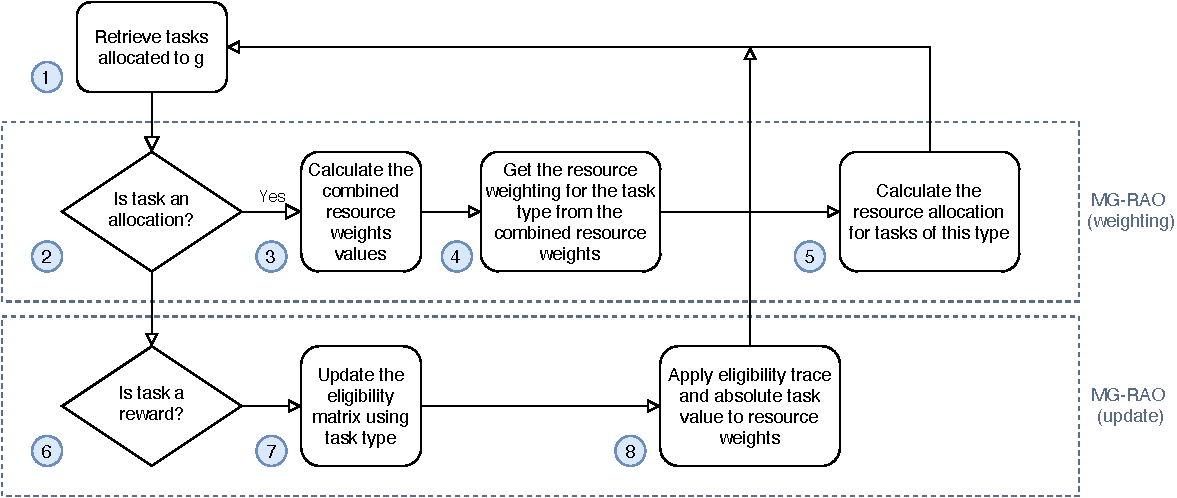
\includegraphics[width=0.8\linewidth, trim={55pt 0pt 55pt 0pt, clip}]{mgrao-simplified}
	\caption{\textbf{Simplified \acronymMGRAO{}{} flowchart}. The diagram shows the decision-making and actions taken by an agent using the \acronymMGRAO{}{}  algorithm. This is a combination of two sub-algorithms, \acronymMGRAO{}{}(weighting), that returns the amount of the agents' resources that are allocated to completing the requested task type, and  \acronymMGRAO{}{}(update), that updates its resource weightings from rewards for previous atomic task completions.}
	\label{fig:mgrao-simplified}
\end{figure}
